% Options for packages loaded elsewhere
\PassOptionsToPackage{unicode}{hyperref}
\PassOptionsToPackage{hyphens}{url}
\PassOptionsToPackage{dvipsnames,svgnames,x11names}{xcolor}
%
\documentclass[
  authoryear,
  preprint,
  3p]{elsarticle}

\usepackage{amsmath,amssymb}
\usepackage{iftex}
\ifPDFTeX
  \usepackage[T1]{fontenc}
  \usepackage[utf8]{inputenc}
  \usepackage{textcomp} % provide euro and other symbols
\else % if luatex or xetex
  \usepackage{unicode-math}
  \defaultfontfeatures{Scale=MatchLowercase}
  \defaultfontfeatures[\rmfamily]{Ligatures=TeX,Scale=1}
\fi
\usepackage{lmodern}
\ifPDFTeX\else  
    % xetex/luatex font selection
\fi
% Use upquote if available, for straight quotes in verbatim environments
\IfFileExists{upquote.sty}{\usepackage{upquote}}{}
\IfFileExists{microtype.sty}{% use microtype if available
  \usepackage[]{microtype}
  \UseMicrotypeSet[protrusion]{basicmath} % disable protrusion for tt fonts
}{}
\makeatletter
\@ifundefined{KOMAClassName}{% if non-KOMA class
  \IfFileExists{parskip.sty}{%
    \usepackage{parskip}
  }{% else
    \setlength{\parindent}{0pt}
    \setlength{\parskip}{6pt plus 2pt minus 1pt}}
}{% if KOMA class
  \KOMAoptions{parskip=half}}
\makeatother
\usepackage{xcolor}
\setlength{\emergencystretch}{3em} % prevent overfull lines
\setcounter{secnumdepth}{5}
% Make \paragraph and \subparagraph free-standing
\ifx\paragraph\undefined\else
  \let\oldparagraph\paragraph
  \renewcommand{\paragraph}[1]{\oldparagraph{#1}\mbox{}}
\fi
\ifx\subparagraph\undefined\else
  \let\oldsubparagraph\subparagraph
  \renewcommand{\subparagraph}[1]{\oldsubparagraph{#1}\mbox{}}
\fi


\providecommand{\tightlist}{%
  \setlength{\itemsep}{0pt}\setlength{\parskip}{0pt}}\usepackage{longtable,booktabs,array}
\usepackage{calc} % for calculating minipage widths
% Correct order of tables after \paragraph or \subparagraph
\usepackage{etoolbox}
\makeatletter
\patchcmd\longtable{\par}{\if@noskipsec\mbox{}\fi\par}{}{}
\makeatother
% Allow footnotes in longtable head/foot
\IfFileExists{footnotehyper.sty}{\usepackage{footnotehyper}}{\usepackage{footnote}}
\makesavenoteenv{longtable}
\usepackage{graphicx}
\makeatletter
\def\maxwidth{\ifdim\Gin@nat@width>\linewidth\linewidth\else\Gin@nat@width\fi}
\def\maxheight{\ifdim\Gin@nat@height>\textheight\textheight\else\Gin@nat@height\fi}
\makeatother
% Scale images if necessary, so that they will not overflow the page
% margins by default, and it is still possible to overwrite the defaults
% using explicit options in \includegraphics[width, height, ...]{}
\setkeys{Gin}{width=\maxwidth,height=\maxheight,keepaspectratio}
% Set default figure placement to htbp
\makeatletter
\def\fps@figure{htbp}
\makeatother

\makeatletter
\@ifpackageloaded{caption}{}{\usepackage{caption}}
\AtBeginDocument{%
\ifdefined\contentsname
  \renewcommand*\contentsname{Table of contents}
\else
  \newcommand\contentsname{Table of contents}
\fi
\ifdefined\listfigurename
  \renewcommand*\listfigurename{List of Figures}
\else
  \newcommand\listfigurename{List of Figures}
\fi
\ifdefined\listtablename
  \renewcommand*\listtablename{List of Tables}
\else
  \newcommand\listtablename{List of Tables}
\fi
\ifdefined\figurename
  \renewcommand*\figurename{Figure}
\else
  \newcommand\figurename{Figure}
\fi
\ifdefined\tablename
  \renewcommand*\tablename{Table}
\else
  \newcommand\tablename{Table}
\fi
}
\@ifpackageloaded{float}{}{\usepackage{float}}
\floatstyle{ruled}
\@ifundefined{c@chapter}{\newfloat{codelisting}{h}{lop}}{\newfloat{codelisting}{h}{lop}[chapter]}
\floatname{codelisting}{Listing}
\newcommand*\listoflistings{\listof{codelisting}{List of Listings}}
\makeatother
\makeatletter
\makeatother
\makeatletter
\@ifpackageloaded{caption}{}{\usepackage{caption}}
\@ifpackageloaded{subcaption}{}{\usepackage{subcaption}}
\makeatother
\journal{Palaeo3}
\ifLuaTeX
  \usepackage{selnolig}  % disable illegal ligatures
\fi
\usepackage[]{natbib}
\bibliographystyle{elsarticle-harv}
\usepackage{bookmark}

\IfFileExists{xurl.sty}{\usepackage{xurl}}{} % add URL line breaks if available
\urlstyle{same} % disable monospaced font for URLs
\hypersetup{
  pdftitle={Interspecies comparisons of Mg/Ca ratios in limpet shells},
  pdfauthor={Niklas Hausmann; Donna Surge; Francisco Zangrando; Angelica Tivoli; Ivan Briz-Godino},
  pdfkeywords={Sclerochronology, Limpets, Elemental Ratio, Mg/Ca},
  colorlinks=true,
  linkcolor={blue},
  filecolor={Maroon},
  citecolor={Blue},
  urlcolor={Blue},
  pdfcreator={LaTeX via pandoc}}

\setlength{\parindent}{6pt}
\begin{document}

\begin{frontmatter}
\title{Interspecies comparisons of Mg/Ca ratios in limpet shells}
\author[1]{Niklas Hausmann%
\corref{cor1}%
}
 \ead{niklas@palaeo.eu} 
\author[2]{Donna Surge%
%
}

\author[3]{Francisco Zangrando%
%
}

\author[3]{Angelica Tivoli%
%
}

\author[4]{Ivan Briz-Godino%
%
}


\affiliation[1]{organization={Leibniz Zentrum für
Archäologie},addressline={Ludwig-Lindenschmit-Forum
1},city={Mainz},country={Germany},countrysep={,},postcode={55116},postcodesep={}}
\affiliation[2]{organization={University of North
Carolina},addressline={104 South Road, 225 Geology
Building},city={Chapel Hill,
NC},country={US},countrysep={,},postcode={27599-3315},postcodesep={}}
\affiliation[3]{organization={CONICET (Consejo Nacional de
Investigaciones Científicas y Técnicas)},addressline={Avenida Maipú
305},city={Ushuaia},country={Argentina},countrysep={,},postcode={V9410BJA},postcodesep={}}
\affiliation[4]{organization={},country={Spain},countrysep={,},postcodesep={}}

\cortext[cor1]{Corresponding author}





        
\begin{abstract}
This document is a template demonstrating the Aps format.
\end{abstract}





\begin{keyword}
    Sclerochronology \sep Limpets \sep Elemental Ratio \sep 
    Mg/Ca
\end{keyword}
\end{frontmatter}
    
\section{Introduction}\label{Introduction}

This study provides a short reassessment of the use of Magnesium to
Calcium (Mg/Ca) ratios in Atlantic limpet shells to determine past sea
surface temperatures. While recent studies of particularly
\emph{Patella} sp. in the Mediterranean and Southwest Europe have
provided promising results
\citep{Hausmann2019-fi, Garcia-Escarzaga2015-jc, Garcia-Escarzaga2018-nf}.

In previous studies, various limpet specimens (Patella vulgata, Nacella
magellanica and Nacella odifosdio) have been studied using Mg/Ca with
mixed results. While Patella vulgata along the Spanish shoreline has
since then repeatedly produced reliable correlations between sst and
Mg/Ca ratios, this is not the case for other species.

In this study, we present elemental maps of various such species
together with stable oxygen isotope values for some of the specimens.
Some of these\ldots{}

\section{Methods}\label{Methods}

\section{Results}\label{Results}

\begin{figure}[H]

{\centering 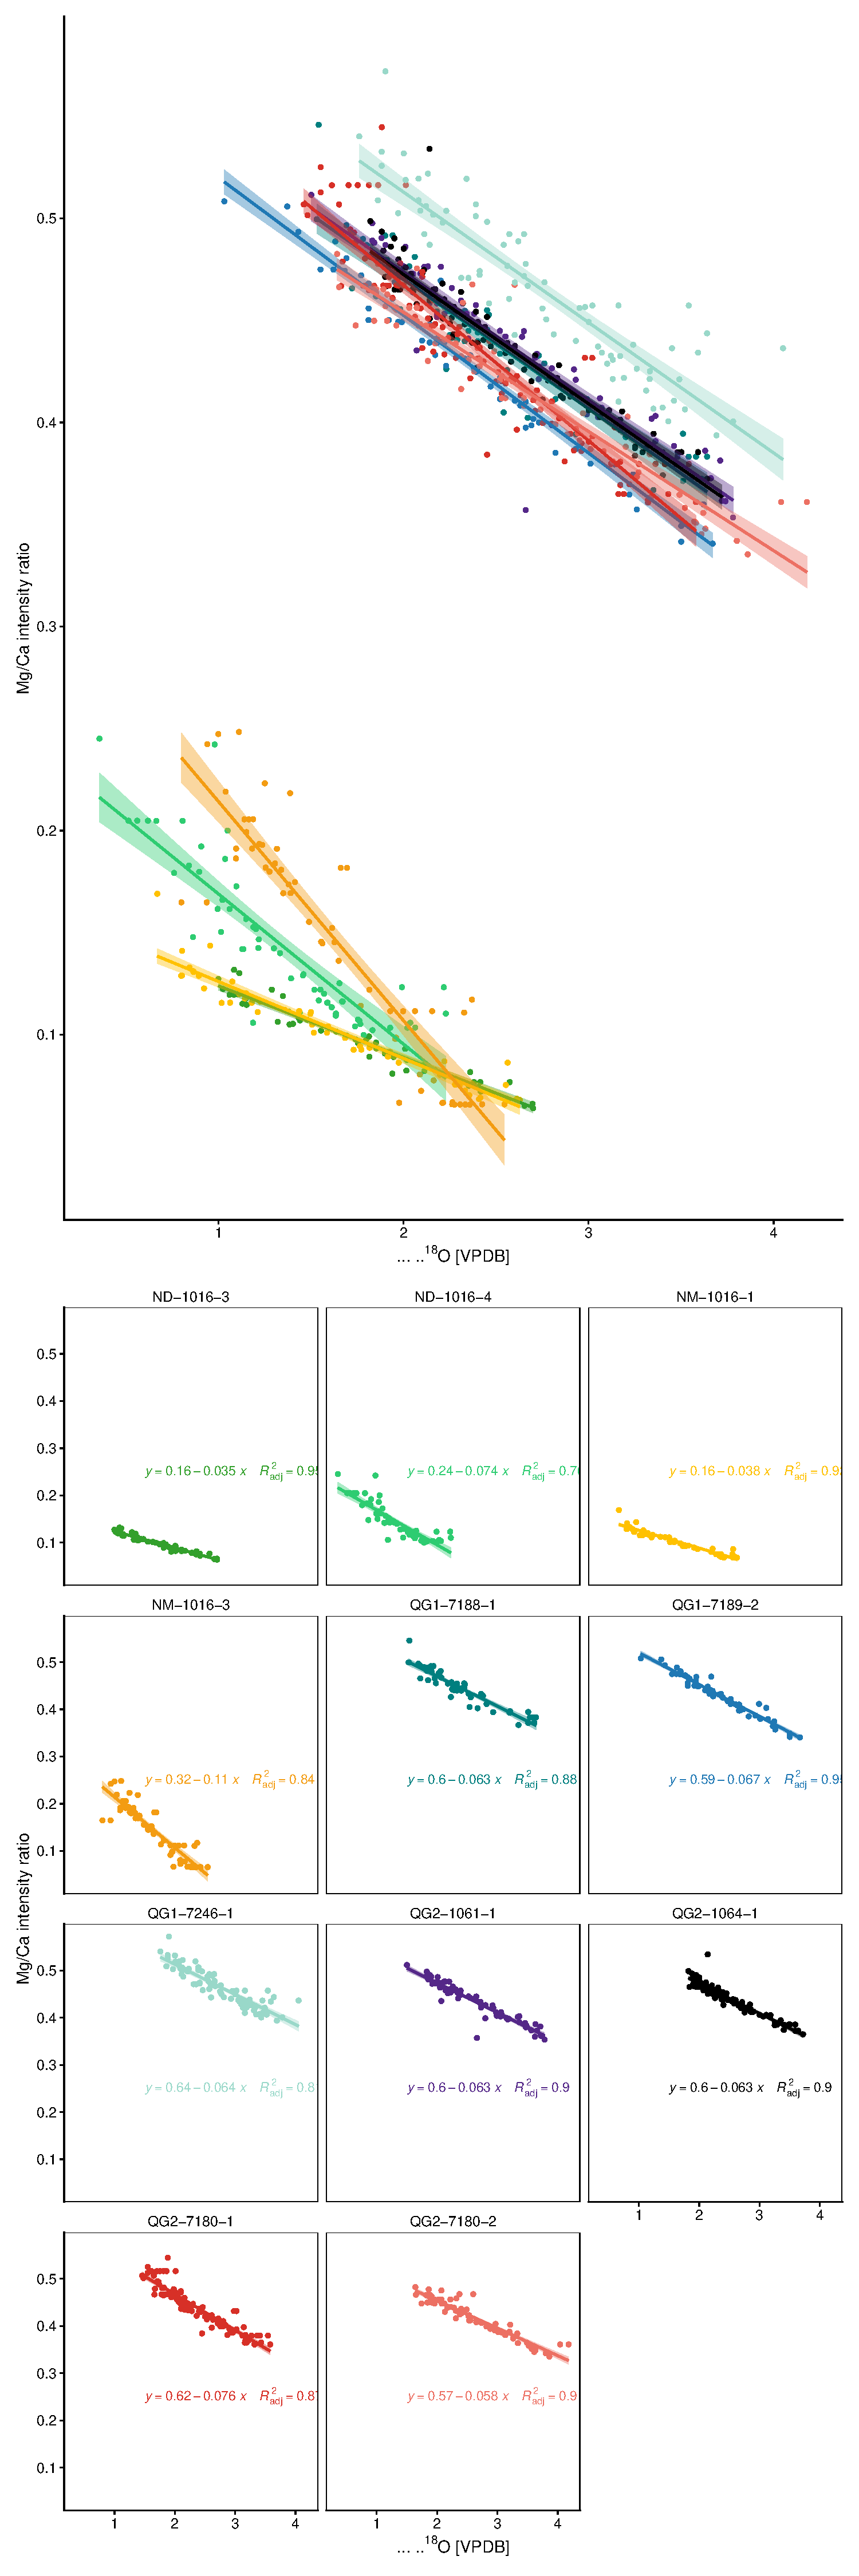
\includegraphics{Manuscript_files/figure-pdf/Correlation Graphs-1.pdf}

}

\caption{Correlation graphs for all specimens}

\end{figure}%

\section{Discussion}\label{discussion}

\begin{figure}[H]

{\centering 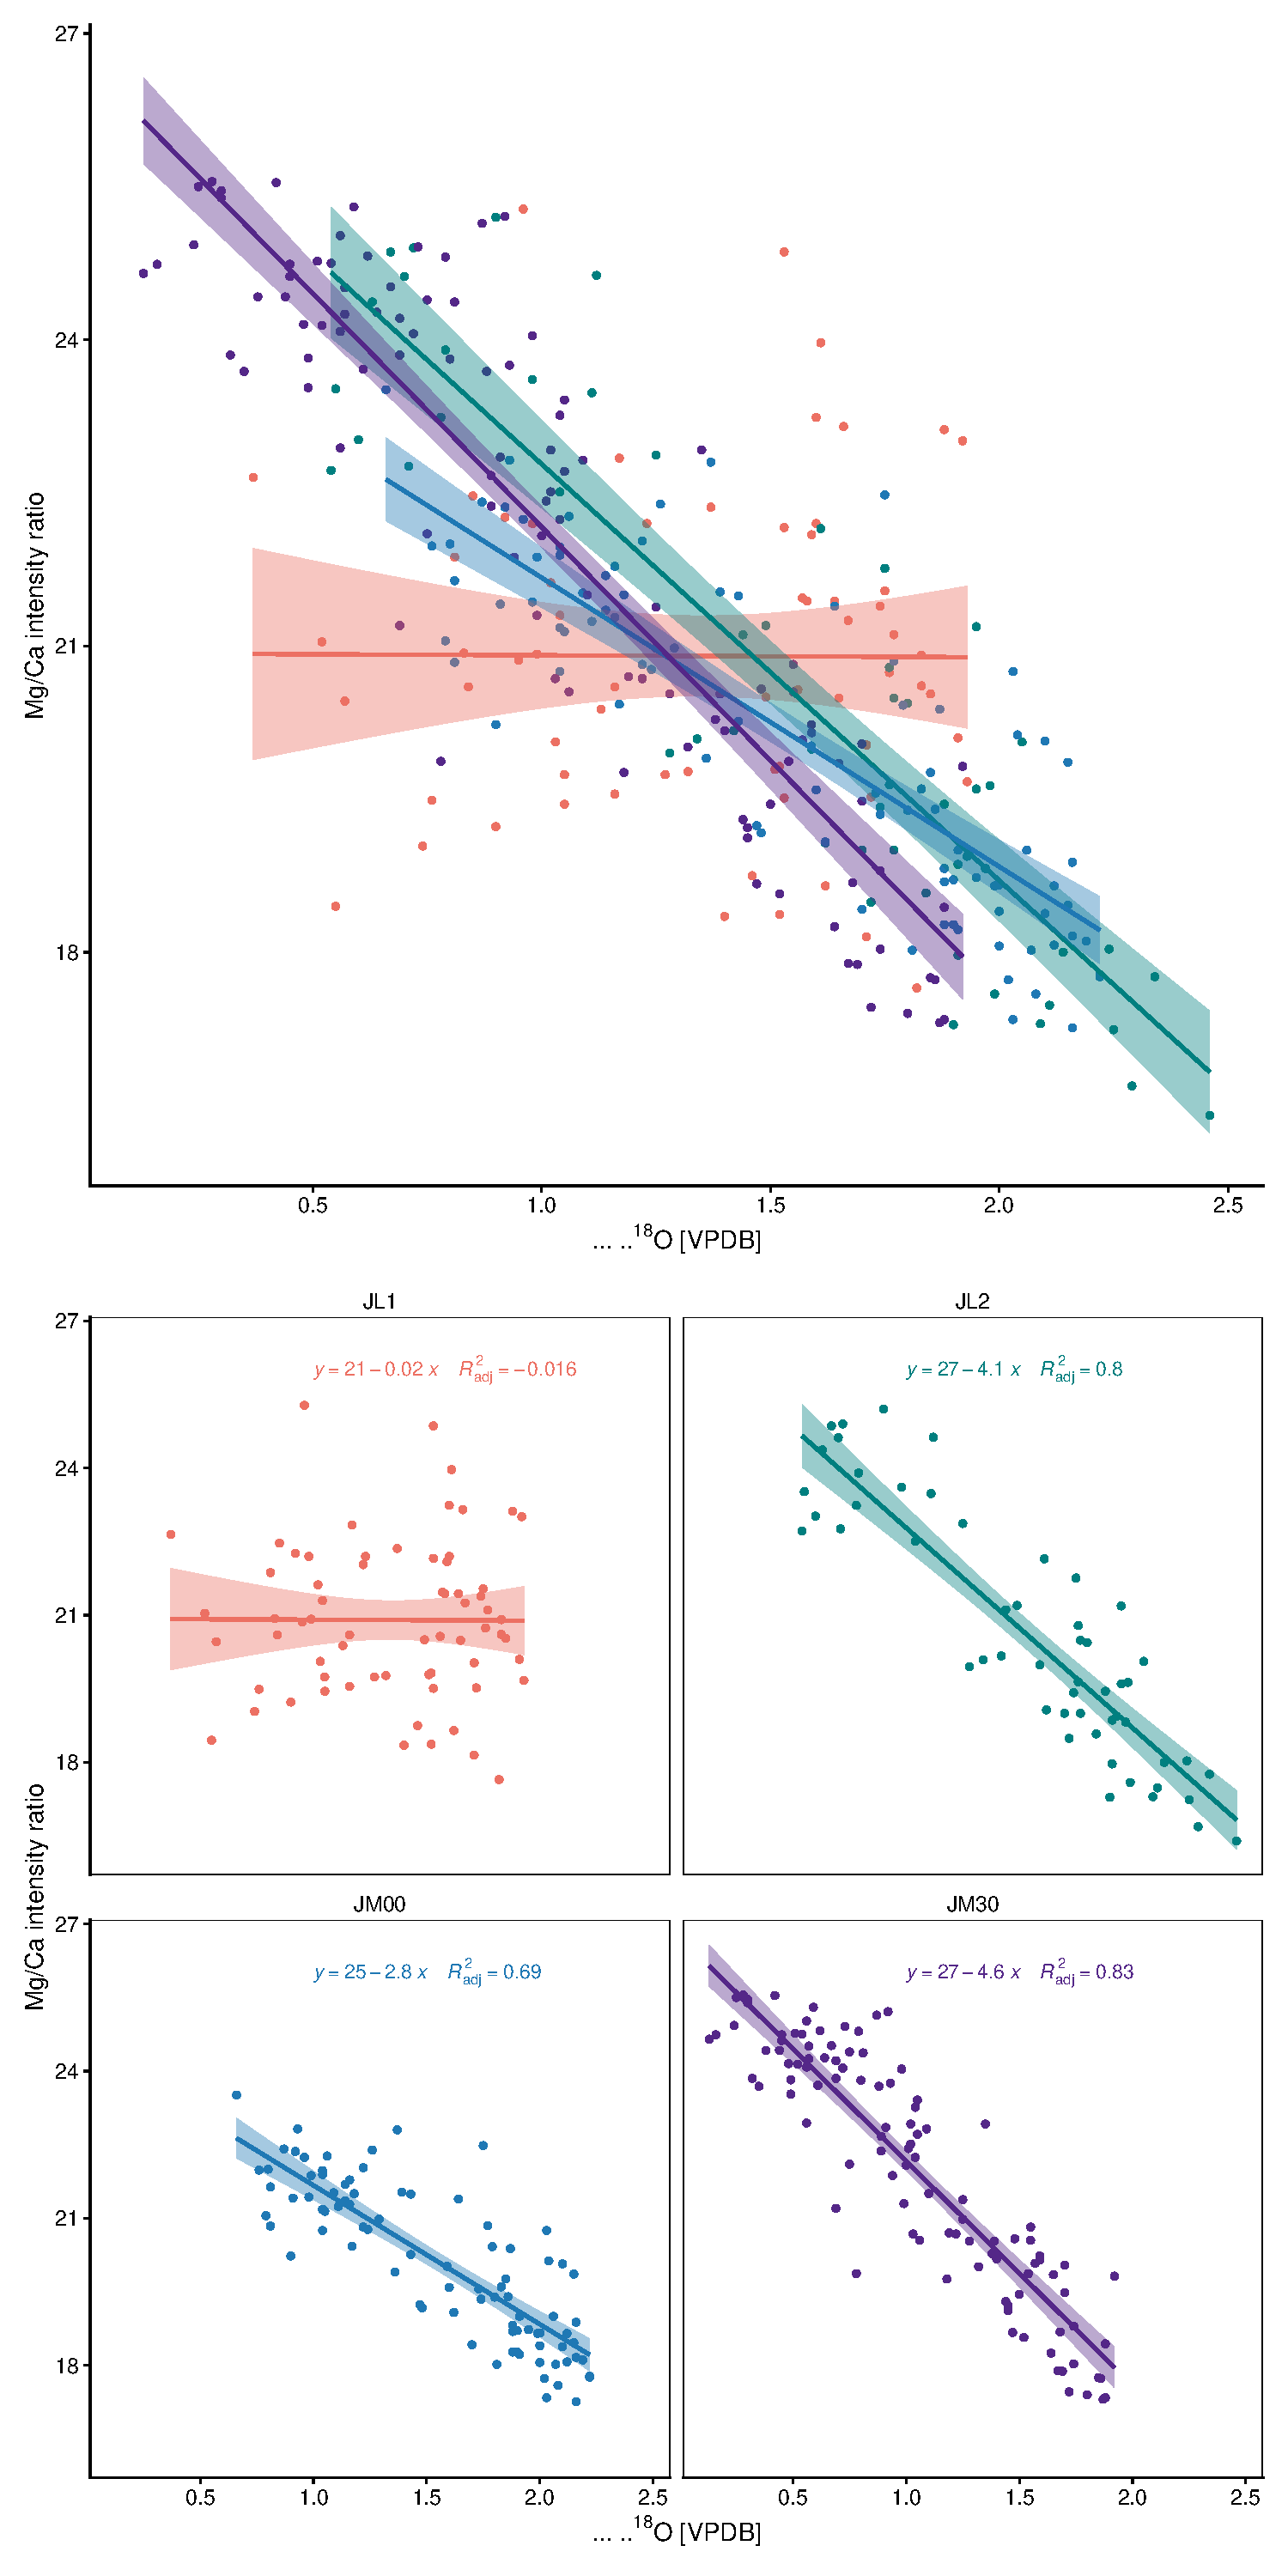
\includegraphics{Manuscript_files/figure-pdf/Ferguson Data-1.pdf}

}

\caption{Correlation graphs for Ferguson et al.~specimens}

\end{figure}%

\begin{longtable}[]{@{}
  >{\raggedright\arraybackslash}p{(\columnwidth - 8\tabcolsep) * \real{0.1528}}
  >{\raggedright\arraybackslash}p{(\columnwidth - 8\tabcolsep) * \real{0.1528}}
  >{\raggedright\arraybackslash}p{(\columnwidth - 8\tabcolsep) * \real{0.1528}}
  >{\raggedright\arraybackslash}p{(\columnwidth - 8\tabcolsep) * \real{0.1528}}
  >{\raggedright\arraybackslash}p{(\columnwidth - 8\tabcolsep) * \real{0.3889}}@{}}
\caption{Overview of comparative correlations
\{\#tab:correlations\}}\tabularnewline
\toprule\noalign{}
\begin{minipage}[b]{\linewidth}\raggedright
Species
\end{minipage} & \begin{minipage}[b]{\linewidth}\raggedright
Locality
\end{minipage} & \begin{minipage}[b]{\linewidth}\raggedright
Specimen
\end{minipage} & \begin{minipage}[b]{\linewidth}\raggedright
Correlation R\textsuperscript{2}
\end{minipage} & \begin{minipage}[b]{\linewidth}\raggedright
Study
\end{minipage} \\
\midrule\noalign{}
\endfirsthead
\toprule\noalign{}
\begin{minipage}[b]{\linewidth}\raggedright
Species
\end{minipage} & \begin{minipage}[b]{\linewidth}\raggedright
Locality
\end{minipage} & \begin{minipage}[b]{\linewidth}\raggedright
Specimen
\end{minipage} & \begin{minipage}[b]{\linewidth}\raggedright
Correlation R\textsuperscript{2}
\end{minipage} & \begin{minipage}[b]{\linewidth}\raggedright
Study
\end{minipage} \\
\midrule\noalign{}
\endhead
\bottomrule\noalign{}
\endlastfoot
\emph{Patella depressa} & Northern Spain & LAN541 & 0.87 &
\href{https://doi.org/10.3390/app11072959}{\textbf{10.3390/app11072959}} \\
& & LAN545 & 0.86 & \\
& & LAN554 & 0.78 & \\
& & LAN559 & 0.82 & \\
\emph{Patella caerulea} & Croatia & ISTPC1 & 0.9 &
10.1038/s41598-019-39959-9 \\
& & ISTPC2 & 0.84 & \\
& Crete & AF1911A & 0.91\footnote{SST only, no other geochemical data
  available} & \\
& & AF3003A & 0.92\footnote{SST only, no geochemical data available}
& \\
& Israel & AKKPC2 & 0.96 & \\
& & AKKPC3 & 0.89 & \\
& & FRMPC1 & 0.84 & \\
& & FRMPC2 & 0.96 & \\
& Libya & MO31A & 0.83 & \\
& & MP64A & 0.33 & \\
& & MP67A & 0.96 & \\
& & MP68A & 0.81 & \\
& Malta & MA10 & 0.82 & \\
& Tunisia & TUNPC1 & 0.81 & \\
& & TUNPC2 & 0.78 & \\
& Turkey & ANTPC1 & 0.95 & \\
& & ANTPC2 & 0.93 & \\
& & KIZPC1 & 0.94 & \\
& & KIZPC2 & 0.86 & \\
Patella rustica & Gibraltar & JL1 & 0.02 &
\href{https://doi.org/10.1016/j.epsl.2011.05.054}{doi.org/10.1016/j.epsl.2011.05.054} \\
& & JL2 & 0.8 (0.79) & \\
Patella caerulea & Gibraltar & JM00 & 0.69 (0.79) & \\
& & JM30 & 0.83 (0.79) & \\
Patella vulgata & Orkney & ORK-LT5 & not reported, here 0.88 &
doi.org/10.1016/j.palaeo.2016.10.021 and this study \\
& & & & \\
& & & & \\
& & & & \\
\end{longtable}

\subsection{Reanalysis of ORK-LT5}\label{reanalysis-of-ork-lt5}

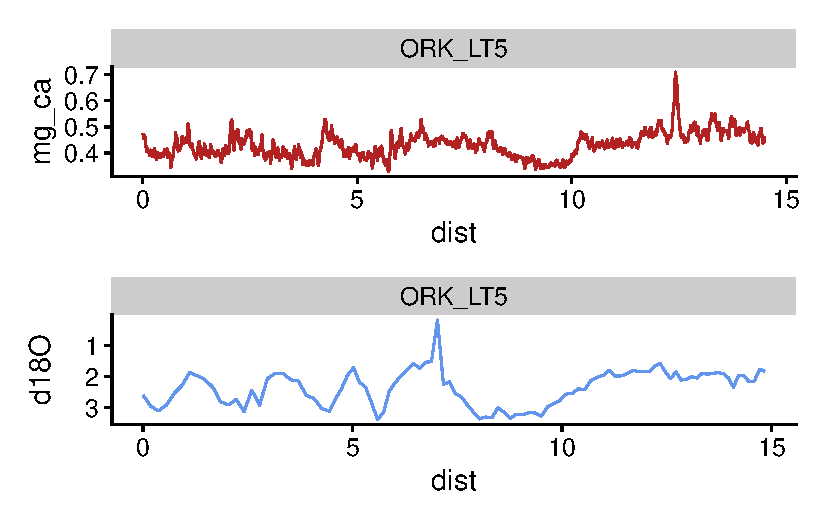
\includegraphics{Manuscript_files/figure-pdf/unnamed-chunk-1-1.pdf}

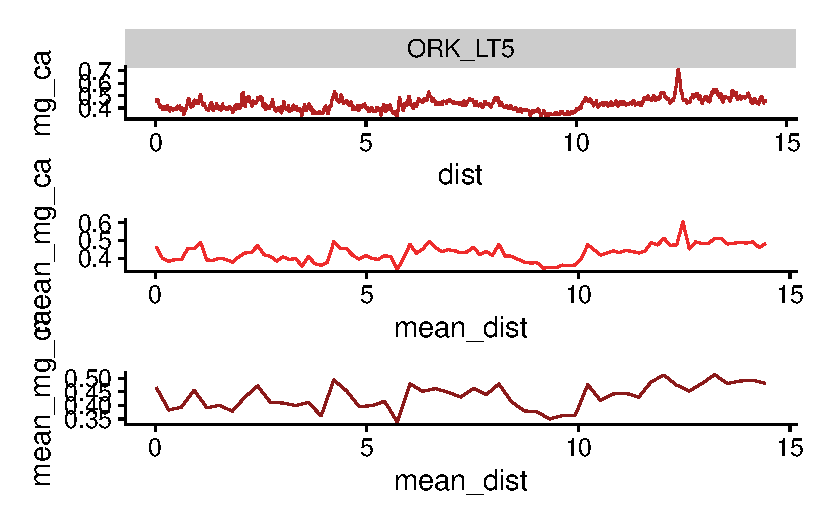
\includegraphics{Manuscript_files/figure-pdf/subsample-1.pdf}


  \bibliography{bibliography.bib}


\end{document}
